\par Now is the time to talk real problems. Constrained optimisation problems are the problems that have constraints. Whenever a problem is restricted to a particular part of the space, we are talking about the constraint optimisation. Remember that the unconstrained and constrained optimisation problems are quite connected. Each constrained problem can be transformed into unconstrained by simply bringing the constraints into the objective function. This can be done with the indicator function: whenever a point does not belong to the admissible region the value of the function goes to $\infty$. No one is that crazy to do it though. The indicator function is a bad function, it brings non differentiability into a problem that may be perfectly differentiable everywhere (both the objective function and the constraints).
\par In general this is a complicated problem unless everything is convex. Most of the times it is but sometimes it is not. Generally the global optimum is very difficult to find. We usually stick to a weaker condition: \textbf{the local optimum $x_*$}:
\begin{equation}
    \min\{f(x) : x \in \mathcal{B}(x_*,\epsilon) \cap X\}
\end{equation}
for some $\epsilon > 0$. Note that we are talking about local optimum, not local minimum. This is not casual. Local minimum is the point where you truly have a minimum of the function. This happens when you are working on the entire space $\mathbb{R}^n$. If you are constrained to a subspace $X$ then you are talking about \textit{minimum in that subspace}. Hence we are talking about the local optimum constrained to that subspace. Clearly, with this definition, if the local optimum is located in the interior of the set $X$, i.e. if $x_* \in \textit{int} X$ then the local optimum is also the local minimum. This is because in the interior of the set the constraints are not touching the optimal solution. So the optimum is independent from the constraints. So in order to have local minimum different from local optimum, it must be located on the boundary of the set, i.e. $\partial X$. So the boundary of the feasible set is quite important.
%
\section{A simple case: feasible sets with no interior}
\par Let us start with the simplest constrained problem: quadratic problem. The problems of this kind are those that have quadratic objective function but linear constraints. Moreover, let us consider a problem with just the linear equality constraints:
\begin{equation}
    \min\{f(x) : Ax = b\}
\end{equation}
where $A \in \mathbb{R}^{m \times n}$ with rank$(A) = m < n$ and rows linearly independent. We need to have more variables than equations because if $m = n$, then it is a square system and thus we could just apply the closed formula and solve it without any fancy optimisation technique. Linear independence is needed because otherwise if there is a row that is linearly dependent from the others then either the system is impossible or that dependant row can be eliminated (linear algebra). Think of a plane that is parallel to another one. In that case, the two planes will never intersect thus there is no solutions.
\par Actually we could transform this particular constrained problem into the unconstrained one. Since $A$ is short and fat, we can split it in two parts: $A_B$ and $A_N$, respectively $m \times m$ matrix and $m \times (n-m)$ matrix. We do the same for the input vector $x$, i.e. $x_B$ of $m$ entries and $x_N$ of $n-m$ entries. So we have:
\begin{equation}
    A_B x_B + A_N x_N = b
\end{equation}
Now if $A_B$ is invertible, that is if det$(A_B) \neq 0$ then we can write the above equation as:
\begin{equation}
    x_B = A_B^{-1}(b - A_N x_N)
\end{equation}
This means that we have transformed the variables of $x_B$ into dependant variables from independent variables $x_N$. In other words, now we con concentrate on optimising just $x_N$, while $x_B$ can be subsequently obtained from $x_N$. How? Like this:
\begin{equation}
    x_B = -A_B^{-1} A_N x_N + A_B^{-1}b = Dw + d
\end{equation}
where:
\[
D = \left[
  \begin{array}{c}
  -A_B^{-1}A_N \\
  I
  \end{array}
\right],
d = \left[
  \begin{array}{c}
  A_B^{-1}b \\
  0
  \end{array}
\right]
\]
and $w \in \mathbb{R}^{n-m}$. The problem then becomes:
\begin{equation}
    w_* = \min_{w \in \mathbb{R}^{n-m}} \{r(w) = f(Dw + d)\}
\end{equation}
which is clearly an unconstrained optimisation problem in $w$. $m$ linear constraints kill $m$ degrees of freedom.
\par We can thus construct a \textit{reduced gradient} of the form:
\begin{equation}
    \nabla r(w) = D^T \nabla f (Dw + d)
\end{equation}
which is obtained by applying the usual derivative of the composition operator (chain rule). How do we solve an unconstrained optimisation problem. The good old gradient: we need to solve:
\begin{equation}
    \nabla r(w_*) = D^T \nabla f (Dw + d) = 0
    \label{eq:chapter3-reduced_gradient}
\end{equation}
\par Let us now explain something that is quite important. We know how to characterise the optimality in the space of $w$. But what happens when we want to write the optimality in the original space of $x$? Note that:
\begin{equation}
    D^T A^T = AD = 0
\end{equation}
Having said that, we can also say that whatever scalar of the matrix $A$ will also produce 0 when multiplied with $D$ (obviously), that is:
\begin{equation}
    \mu AD = \mu D^T A^T = 0
\end{equation}
Let us now call $\mu A$ with $z$:
\begin{equation}
    D^T z = 0
\end{equation}
Now, look at the gradient in \ref{eq:chapter3-reduced_gradient}. We want to find a point $x = Dw + d$ such that the gradient of that point $x$ multiplied with $D^T$ will give us 0. But that would mean:
\begin{equation}
    \mu A = \nabla f(x), x=Dw + d
\end{equation}
So the gradient must be a scalar multiple of $A$. So if we manage to find $x$ such that the gradient of $f$ in that point is a multiple of $A$, then in the space of $w$ that point is a stationary point, and $x$ is a local optimum.
\par Let us now state it in more formal terms:
\begin{equation}
\begin{split}
    &\mbox{if}\\
    &Ax = b \mbox{ and } \exists \mu : \mu A = \nabla f(x)\\
    &\mbox{then}\\
    &x \mbox{ is a stationary point for } (P) \equiv \min \{f(x) : Ax = b\}
\end{split}
\end{equation}
This is a special case of \textbf{Poorman's KKT conditions}, which are THE optimality conditions for constraint optimisation problems. Basically, the optimal point must be a feasible point and the gradient in that point must be written as a linear combination of the gradients of the constraints. So in order to show that $x$ is optimal, we need to compute $\mu$.
\par Of course if $f$ is convex, these conditions are also sufficient for the optimality.
\subsection{Geometric interpretation}
\par What are these $\mu$ geometrically speaking? Suppose you have a quadratic function whose level sets are shown in figure \ref{fig:chapter3-contraint_equality_1}. In the same figure you can also see a line that correspond to the feasible region described by the equality constraints $Ax = b$. For the sake of simplicity, suppose we have just one equality, as in figure. Remember that we are in $\mathbb{R}^n$ space, not $\mathbb{R}^{n+1}$ where the value of the function lives.
\par The minimum is clearly located in the point in the middle of the inner most level set. But since we must restrict the admissible points to the admissible region indicated by $Ax = b$, the local optimum is the point that is the intersection between the line and the inner most level set. Why inner most? Because every other outer level set has a greater function value.
\begin{figure}
    \centering
    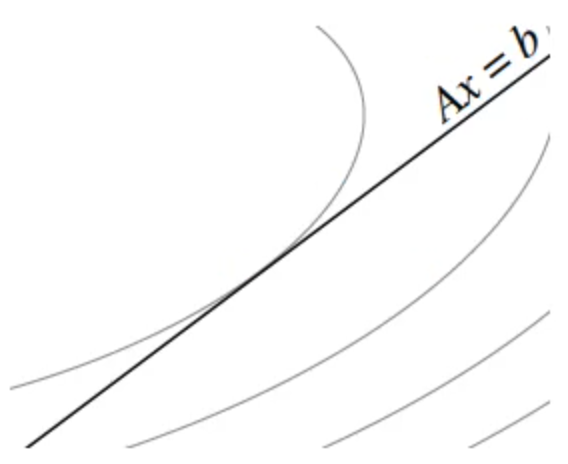
\includegraphics[scale=0.5]{figures/3/chapter3-constraint_equality_1.png}
    \caption{Caption}
    \label{fig:chapter3-contraint_equality_1}
\end{figure}
\par Now, we know that the gradient is always normal (orthogonal) to the level sets. Consequently, it is also normal to the admissible region in the point of the intersection, i.e. $\nabla f(x) \perp \partial X$ (see figure \ref{fig:chapter3-constraint_equality_2}). But since by definition $A \perp \partial X$ (all the points in $X$ have the scalar product 0 with $A$), it must be that the gradient is also co-linear with $A$, i.e. $A \parallel \nabla f(x)$ (see figure \ref{fig:chapter3-constraint_equality_3}).
\begin{figure}
    \centering
    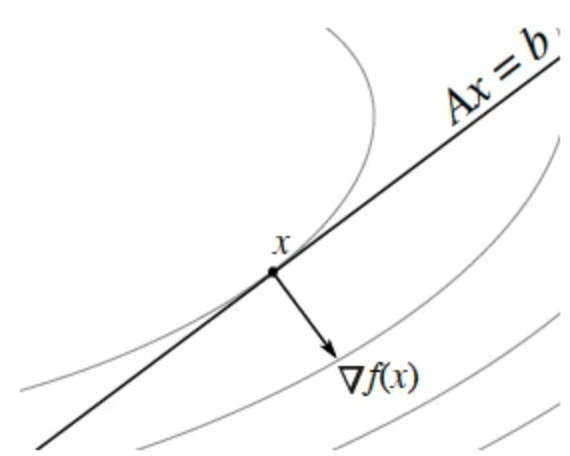
\includegraphics[scale=0.5]{figures/3/chapter3-constraint_equality_2.png}
    \caption{Caption}
    \label{fig:chapter3-constraint_equality_2}
\end{figure}
\begin{figure}
    \centering
    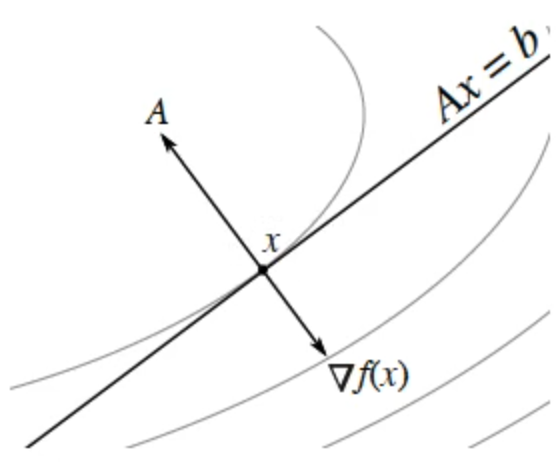
\includegraphics[scale=0.5]{figures/3/chapter3-constraint_equality_3.png}
    \caption{Caption}
    \label{fig:chapter3-constraint_equality_3}
\end{figure}
\par The matrix $A$ sends every vector somewhere in the space, you remember, matrices are used for transformations :). The vectors that when multiplied with $A$ produce $b$ are in the admissible region. But who said $A$ likes only the admissible region? $A$ sends vectors wherever: and so it can send also in the opposite direction. Exactly where our gradient is located.
\par It is for this reason that we define the directions in the feasible region:
\begin{equation}
    F = \{d \in \mathbb{R}^n : A \cdot x = 0\}
\end{equation}
\par In constrained optimisation it is no more necessary to have the gradient zero in the optimal point. Think of taking a minimum of a concave quadratic function whose admissible region is from a certain level set above. Clearly the minimum is at the edge of the admissible region. In that point the gradient is for sure negative.
\par What we have in the local optimum point is that all the directions in the feasible region have the scalar product with the gradient $\geq 0$:
\begin{equation}
    \nabla f(x) \cdot d \geq 0, \forall d \in F
\end{equation}
\par Unfortunately constraints are way more complicated than lines and affine spaces. So we need to dive into it, right now.
%
\section{The theory of ice creams: cones}
\par The crucial mathematical object that we are going to use to define the optimality is the \textbf{Tangent Cone}:
\begin{equation}
    T_X(x) = \Big\{d \in \mathbb{R}^n : \exists \{z_i \in X\} \rightarrow x \wedge \{t_i \geq 0\} \rightarrow 0 : d = \lim_{i \rightarrow \infty} \frac{z_i-x}{t_i}\Big\}
\end{equation}
\par Err... what? Yes, it is not nice as a definition. But it is easier than you think. Basically, this definition states that in order for $d$ to be a direction along which we can move from the current point $x$, it must be a direction that comes from a sequence of points belonging to the feasible set and that converge to $x$. But also there must be a sequence of corresponding step sizes that converge to 0. The overall sequence may be a straight line, may be of sinusoidal form, it may even be on the border. What matters is that it tends to $x$ in the limit \ref{fig:chapter3-tangent_cone}.
\begin{figure}
    \centering
    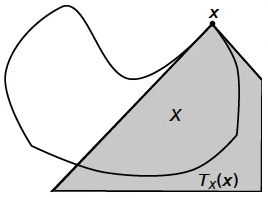
\includegraphics[scale=0.5]{figures/3/chapter3-tangent_cone.png}
    \caption{An example of the tangent cone}
    \label{fig:chapter3-tangent_cone}
\end{figure}
\par Why is this cone important? Because it provides a necessary condition for $x$ to be local optimum (and global optimum in case $X$ is convex).
\begin{theorem}
    \[x \mbox{ local optimum } \Rightarrow \nabla f(x) \cdot d \geq 0, \forall d \in T_X(x)\]
\end{theorem}
\begin{proof}
    Let us assume by contradiction that there exists a direction in the local optimum $x$ that has negative scalar product with the gradient of $x$. Let us call that direction $d$. Since $d \in T_X(x)$, this means that there exists a sequence of points $\{z_i\}$ in $X$ that converge to $x$ with a sequence of step sizes $\{t_i\}$ that converge to 0. Consider now the first order Taylor expansion in $z_i$:
    \begin{equation}
        \begin{split}
            f(z_i) &= f(x) + \nabla f(x)(z_i - x) + R(z_i - x) =\\
            &= f(x) + \nabla f(x) \cdot (z_i - x) + R(z_i - x)
        \end{split}
    \end{equation}
    Let us now add $-f(x)$ to both sides, divide them by $t_i$ and send them to limit:
    \begin{equation}
        \begin{split}
            \lim_{i \rightarrow \infty} \frac{f(z_i) - f(x)}{t_i} &= \nabla f(x) \cdot \lim_{i \rightarrow \infty} \frac{z_i - x}{t_i} + \lim_{i \rightarrow \infty} \frac{R(z_i - x)}{t_i} =\\
            &=\nabla f(x) \cdot   d + \lim_{i \rightarrow \infty} \frac{R(z_i - x)}{t_i} < 0
        \end{split}
    \end{equation}
    Which is a contradiction. The scalar product is negative by assumption and the limit on the right is converging to 0. So the whole right part is strictly negative. This would mean that $z_i$ is a point in the neighbour of $x$ that has the value of the function strictly smaller than the one in $x$. But we said that $x$ was a local optimum.
\end{proof}
\par Something that you could say: yes but if $x$ is local optimum, nobody is telling me that it is also a global optimum. Thus, for sufficiently large ball around $x$, I could find a point where the function value is actually smaller than the one in $x$. True. But we are talking about cones, not balls. There must not be a point in the cone of $x$ that has a smaller value.
\par Tangent cone does not give us also the sufficient condition. In other words, there may be a point $y$ where all the directions in the tangent cone of $y$ give positive scalar product with the gradient $\nabla f(y)$, but still $y$ may not be a local optimum.
\par Consider the example in figure \ref{fig:chapter3-tangent_cone_not_sufficient1}. This function is clearly not convex. The grey part is the admissible region $X$. Consider the point $x$ in the origin as our current point. The set of directions that are part of the tangent cone in $x$ are all those directions that belong to the positive part of the $y$ axe (see figure \ref{fig:chapter3-tangent_cone_not_sufficient2}). All those directions give $\geq 0$ scalar product with the gradient in $x$. Clearly, the point $x$ is not a local optimum. $x$ is just a stationary point.
\begin{figure}
    \centering
    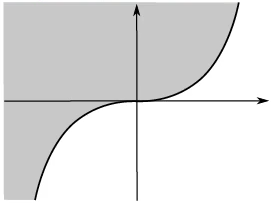
\includegraphics[scale=0.5]{figures/3/chapter3-tangent_cone_not_sufficient1.png}
    \caption{A counterexample for the sufficient condition of the tangent cone.}
    \label{fig:chapter3-tangent_cone_not_sufficient1}
\end{figure}
\begin{figure}
    \centering
    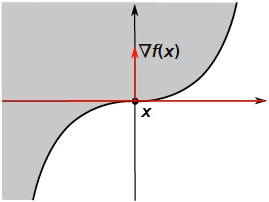
\includegraphics[scale=0.5]{figures/3/chapter3-tangent_cone_not_sufficient2.png}
    \caption{$T_X(x)$ is the $x$ axes. All directions are in 0 scalar product with the gradient $\nabla f(x)$.}
    \label{fig:chapter3-tangent_cone_not_sufficient2}
\end{figure}
\par What we really want to have is the set of feasible directions.
\begin{equation}
    F_X(x) = \{d \in \mathbb{R}^n : \exists \bar \epsilon > 0 \mbox{ s.t. } x + \epsilon d \in X, \forall \epsilon \in [0,\bar \epsilon]\}
\end{equation}
\par If $X$ is convex we can omit the last part of the definition and just use $\bar \epsilon$ instead of $\epsilon$.
\par Clearly, this cone looks very similar to the tangent cone. Generally, the feasible directions cone is not a closed set ($T_X$ is). The closure of $F_X$ is always a subset of $T_X$ and if everything is convex then the closure of $F_X$ is the very same $T_X$. In this case we could actually conclude that:
\begin{equation}
    x \mbox{ is global optimum } \iff \nabla f(x) \cdot d \geq 0, \forall d \in T_X(x)
\end{equation}
\par How do we characterise $T_X$? It depends on how you characterise the admissible region $X$. Usually, one can do that in many different ways. A classical way is by explicitly describing the constraints:
\begin{equation}
    X = \{x \in \mathbb{R}^n : g_i(x) \leq 0, i \in \mathcal{I}, h_j(x) = 0, j \in \mathcal{J}\} = \{x \in \mathbb{R}^n : G(x) \leq 0, H(x) = 0\}
\end{equation}
where $\mathcal{I}$ is the set of inequalities and $\mathcal{J}$ is the set of equalities. Note that $G$ and $H$ are vector valued functions. $G$ sends vectors from space $\mathbb{R}^n$ to vectors in space $\mathbb{R}^{|\mathcal{I}|}$ and $H$ sends vectors from space $\mathbb{R}^n$ to vectors in space $\mathcal{R}^{|\mathcal{J}|}$.
\par There is a nice \textit{theoretical} way to represent all the constraints with just one inequality constraint. To do that, we need to passages:
\begin{itemize}
    \item Each equality constraint can be expressed as two inequality constraints:
    \[a = 0 \iff a \leq 0 \wedge -a \leq 0\]
    \item The set of inequality constraints follows the relation:
    \[G(x) \leq 0 \iff \max\{g_i(x) : i \in \mathcal{I}\} \leq 0\]
\end{itemize}
\par One concept that we will use a lot is the set of \textbf{active constraints}. A constraint is active if the point is on the border described by that constraint. By definition all the equality constraint are always active, otherwise the point would not be in the feasible region. The active inequality constraints are basically all those constraints that result in $=0$. In formulae:
\begin{equation}
    \mathcal{A}(x) = \{i \in \mathcal{I} : g_i(x) = 0\}
\end{equation}
It is thus convenient to define $G$ restricted to that particular set of indices whose corresponding inequalities are active:
\begin{equation}
    G_{\mathcal{A}(x)} : \mathbb{R}^n \rightarrow \mathbb{R}^{|\mathcal{A}(x)|}
\end{equation}
\par So now we can define a cone that can be used in practical way. The cone is called \textbf{first order feasible direction cone}.
\begin{equation}
    D_X(x) = \{d \in \mathbb{R}^n : \nabla g_i(x) \cdot d \leq 0\ i \in A(x), \nabla h_j(x) \cdot d  = 0\ j \in \mathcal{J}\}
\end{equation}
Note that we are now looking into the gradients not functions. It is for this reason that we can rewrite the above definition with:
\begin{equation}
    D_X(x) = \{d \in \mathbb{R}^n : JG_{A(x)}(x) \cdot d \leq 0, JH(x) \cdot d = 0\}
\end{equation}
where $J$ stands for Jacobian matrix.
\par Each active inequality $i$ defines one particular curve that passes in the point $x$. The gradient in $x$ with respect to that curve will be normal to the curve it self (see figure \ref{fig:chapter3-feasible_cone} for an example).
\begin{figure}
    \begin{subfigure}{0.31\textwidth}
        \centering
        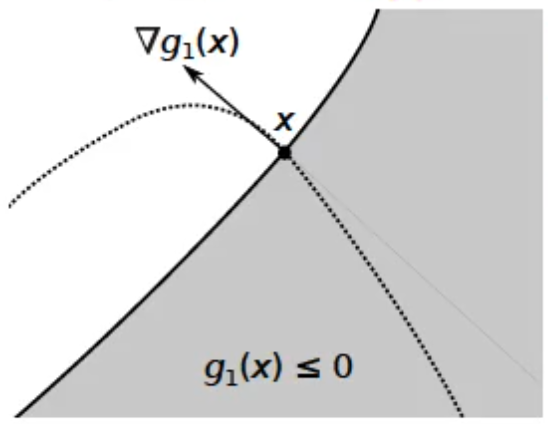
\includegraphics[width=\linewidth]{figures/3/chapter3-feasible_cone1.png}
        \caption{Caption}
        \label{fig:feasible1}
    \end{subfigure}
    \begin{subfigure}{0.31\textwidth}
        \centering
        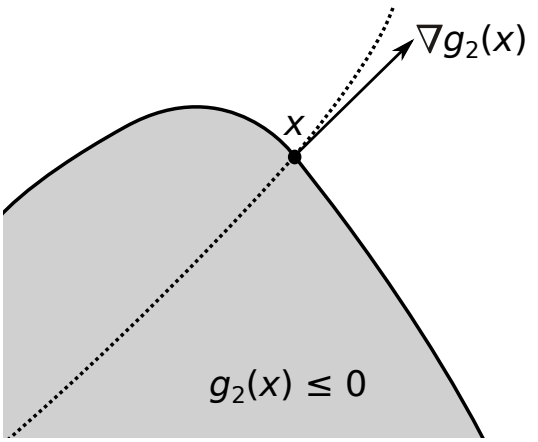
\includegraphics[width=\linewidth]{figures/3/chapter3-feasible_cone2.png}
        \caption{Caption}
        \label{fig:feasible2}
    \end{subfigure}
    \begin{subfigure}{0.31\textwidth}
        \centering
        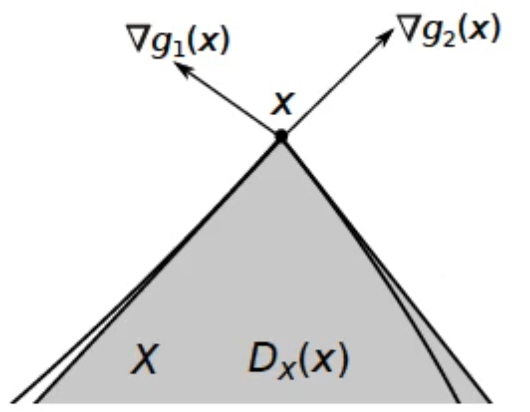
\includegraphics[width=\linewidth]{figures/3/chapter3-feasible_cone3.png}
        \caption{Caption}
        \label{fig:feasible3}
    \end{subfigure}
    \caption{Assume we have only two active inequalities in the point $x$. Take the two corresponding gradients and then construct the cone in the opposite direction.}
    \label{fig:chapter3-feasible_cone}
\end{figure}
\par It is intuitive that the tangent cone is contained in the first order feasible directions cone, i.e.:
\begin{equation}
    T_X(x) \subseteq D_X(x)
\end{equation}
\par So what we really want is the set of feasible directions $F_X$, but due to the closure issue we moved to the tangent cone directions $T_X$, and finally due to its complexity of characterisation we have constructed the first order feasible directions cone $D_X$. It is clear that all of these cones are very similar to each other. We would like to have the tangent cone same as the first order feasible directions cone. Unfortunately, in some pathological cases this may not be true. In other words, we could have $T_X \subset D_X$ (see figure \ref{fig:chapter3-feasible_cone_larger}).
\begin{figure}
    \centering
    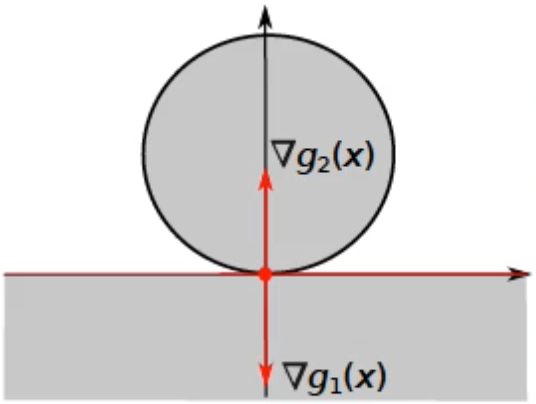
\includegraphics[scale=0.6]{figures/3/chapter3-feasible_cone_larger.png}
    \caption{Suppose you have to convex constraints, one is the all negative subspace of the $y$ axes and the other one is the ball you see in the figure. The first order feasible directions cone is the whole $x$ axes while the tangent cone consist just of one point, the origin. This is because the feasibility region is just the origin (the intersection of the two constraints). $D_X(x) = \{[x_1,x_2] : x_2 = 0\}, T_X(x) = F_X(x) = [0,0]$.}
    \label{fig:chapter3-feasible_cone_larger}
\end{figure}
Note that here everything is convex. So the convexity are not helping us to make the two cones the same stuff.
\par We need to to introduce something that will guarantee us that we are not in some of these pathological cases. This something is called \textit{constraint qualifications}. There are plenty of them, but let us consider the three most important for our purposes:
\begin{itemize}
    \item Affine constraints: everything is linear, except the objective function. It this constraint holds then $\forall x \in X\ T_X(x) = D_X(x)$.
    \item Slater's conditions: inequalities are convex and equalities are affine. If there exists at least one point $x \in X$ that is in the interior, $g_i(x) < 0, \forall i \in \mathcal{I}$, then $T_X(x) = D_X(x), \forall x \in X$. Informally, Slater's condition states that the feasible region must have an interior point.
    \item Linear independence: given a point $x \in X$, if the set of:
    \[
        \{\nabla g_i(x) : i \in \mathcal{I}\} \cup \{h_j(x) : j \in \mathcal{J}\}
    \]
    is linearly independent, then $T_X(x) = D_X(x)$.
\end{itemize}
\par But excluding these pathological cases, or by using some of the constraint qualifications, we have our necessary condition (also sufficient in convex case):
\begin{equation}
    \nabla f(x) \cdot d \geq 0, \forall x \in D_X(x)
\end{equation}
\par The problem is: there are infinitely many directions to check.
%
\subsection{Farkas' lemma}
\par Let us now see how we can avoid checking all the infinite direction of the first order feasible directions cone $D_X$ but still be able to say whether we are in the local optimum or not. We know that $D_X$ is a polyhedral cone of type: $\{d \in \mathbb{R}^n : Ad \leq 0\}$. Now consider the figure \ref{fig:chapter3-farkas1}. Consider a generic vector $c \in \mathcal{R}^n$. This vector can either belong to the dual cone or not. In case it belongs then we can write $c$ as a linear combination of the gradients (see figure \ref{fig:chapter3-farkas2}) . Otherwise there must exist a direction $d$ in the original cone that has a positive scalar product with $c$ (see figure \ref{fig:chapter3-farkas3}).
\begin{figure}
    \centering
    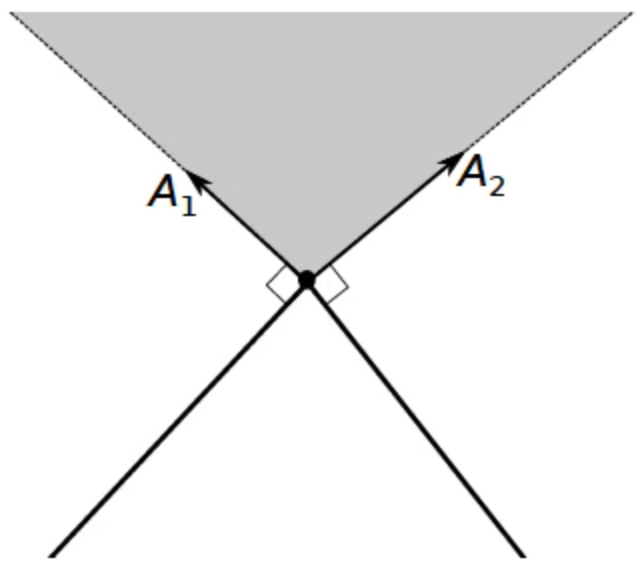
\includegraphics[scale=0.5]{figures/3/chapter3-farkas1.png}
    \caption{The dual cone $C^* = \{c = \sum_{i=1}^k \lambda_i A_i : \lambda_i \geq 0\}$ is the one defined by the two gradients and all the positive linear combinations of the two.}
    \label{fig:chapter3-farkas1}
\end{figure}
\begin{figure}
    \centering
    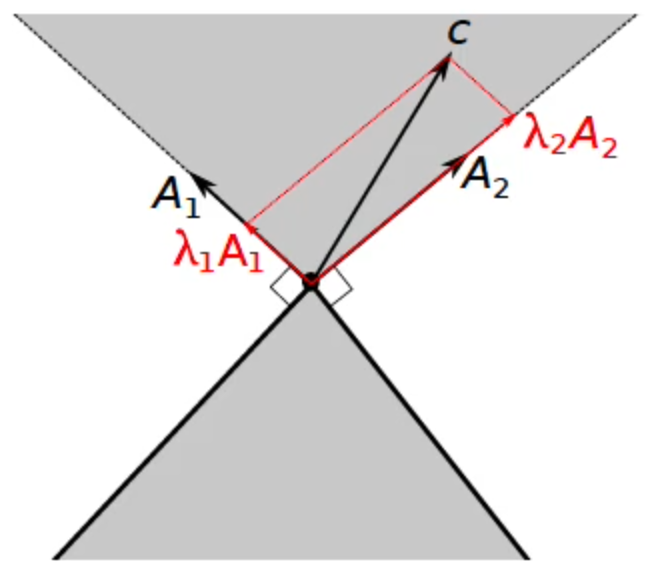
\includegraphics[scale=0.5]{figures/3/chapter3-farkas2.png}
    \caption{If $c \in C^*$ then there must be a set of non negative $\lambda_i$ multipliers for the linear combination of gradients to produce $c$.}
    \label{fig:chapter3-farkas2}
\end{figure}
\begin{figure}
    \centering
    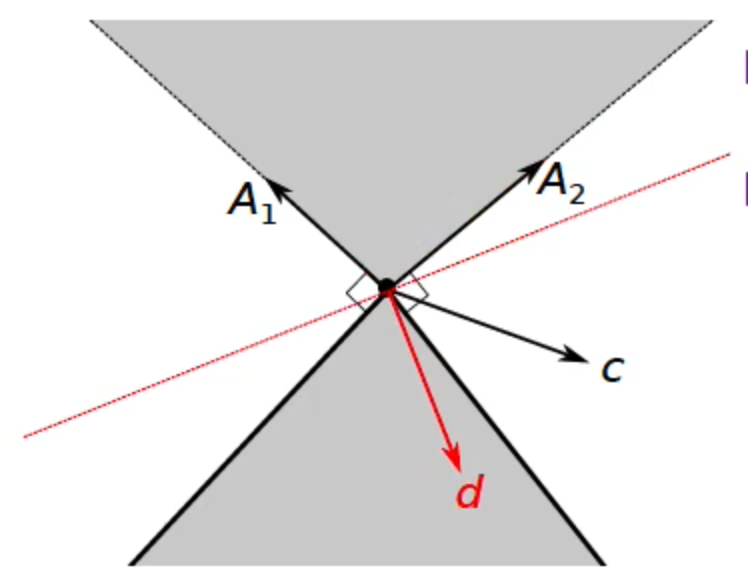
\includegraphics[scale=0.5]{figures/3/chapter3-farkas3.png}
    \caption{If $c \notin C^*$ then it must be the case that there is $d \in C$ such that $c \cdot d > 0$.}
    \label{fig:chapter3-farkas3}
\end{figure}
\par Let us formally define Farkas' lemma:
\begin{theorem}
    \[
        \forall c \in \mathbb{R}^n . \exists \lambda \geq 0 : c = \lambda A \vee \exists d : Ad \leq 0 \wedge c \cdot d > 0
    \]
\end{theorem}
\par Note that we use strictly greater than 0 and not $\geq 0$. This is because if we were using $\geq$ then our vector $c$ could have been $A_2$ for instance.
\par Why do we care about Farkas' lemma? Get ready!
\par We want to use Farkas' lemma to get a nice and (more than everything) useful necessary condition. So we want something like:
\begin{equation}
\begin{split}
    &x^* \mbox{ is local optimum } \Rightarrow \nabla f(x^*) \cdot d \geq 0, \forall d \mbox{ that satisfy: }\\
    &\nabla g_i(x^*) \cdot d \leq 0, \forall i \in \mathcal{A}(x^*) \wedge \nabla h_i(x^*) \cdot d = 0, \forall j \in \mathcal{J}
\end{split}
\end{equation}
\par Turns out that this problem is equivalent to:
\begin{equation}
    \begin{split}
        &x^* \mbox{ is local optimum } \Rightarrow \exists \lambda \in \mathbb{R}_{+}^{|\mathcal{A}(x^*)|} \wedge \mu \in \mathbb{R}^{|\mathcal{J}|} \mbox{ s.t. }\\
        &f(x^*) + \sum_{i \in \mathcal{A}(x^*)} \lambda_i \nabla g_i(x^*) + \sum_{j \in \mathcal{J}} \mu_i \nabla h_j(x^*) = 0
    \end{split}
    \label{eq:chapter3-multipliers}
\end{equation}
Note that we are saying that the opposite of the gradient must be written as the linear combination of the two sums. Moreover, note that we leave $\mu$ to be of any sign. This is not a random stuff. As we know, each equality constraint can be written as two inequality constraints:
\begin{equation}
    \nabla h(x) = 0 \iff \nabla h(x) \leq 0 \wedge -\nabla h(x) \leq 0
\end{equation}
so there exist two positive scalars $\mu^+, \mu^-$ such that:
\begin{equation}
    \mu^+ \nabla h(x) \leq 0 \wedge \mu^- \nabla  h(x) \leq 0
\end{equation}
thus we can write:
\begin{equation}
    (\mu^+ - \mu^-)\nabla h(x) = 0
\end{equation}
This difference can be of any sign.
\par So if $x^*$ is a local optimum then there must exist the multipliers $\lambda$ and $\mu$ such that \ref{eq:chapter3-multipliers} holds. This is a necessary condition (under constraint qualifications), and also sufficient in case of convex optimisation.
%
\subsection{From Farkas' lemma to KKT saint graal}
\par So the equivalent problem from above takes name of \textbf{Karush-Kuhn-Tucker conditions}. The complete characterisation of KKT conditions is the following:
\begin{align}
    &g_i(x) \leq 0, i \in \mathcal{I} \mbox{ and } h_j(x) = 0, j \in \mathcal{J} && \mbox{(KKT-F)}\\
    &\nabla f(x) + \sum_{i \in \mathcal{I}} \lambda_i \nabla g_i(x) + \sum_{j \in \mathcal{J}} \mu_i \nabla h_j(x) = 0 && \mbox{(KKT-G)}\\
    &\sum_{i \in \mathcal{I}} \lambda_i g_i(x) = 0 && \mbox{(KKT-CS)}
\end{align}
The first condition requires that the point $x$ is feasible. The second is the Farkas' lemma stuff, so $-\nabla f(x)$ has to be written as the linear combination of the gradients of the constraints. Note how we are using the whole set of inequalities not just the active ones. This is why we need the third constraint called \textbf{complementary slackness}. Think about it: with complementary slackness constraint, an inequality constraint $i$ is either active, and then $g_i(x) = 0$ so $\lambda$ can be any number; or the constraint $i$ is not active, i.e. $g_i(x) < 0$, but due to the complementary slackness requirement, $\lambda_i$ must be 0.
\par $\lambda$ and $\mu$ are called \textbf{Lagrangian multipliers} or \textbf{Lagrangian} duals.
\par Let us now announce the saint graal of the constraint optimisation:
\begin{theorem}
    If the constraint qualification hold, that is $T_X(x) = D_X(x)$ and $x$ is local optimum, then KKT conditions must hold, that is there must be some $\lambda$ and $\mu$ such that the KKT constraints hold all together.
\end{theorem}
Moreover, under convexity, this theorem becomes if and only if. So in the end, KKT conditions are the ones that recognise the local optimum.
%
\subsection{The nasty critter: Lagrangian function}
\par Let us briefly touch the bad guy: non convex case. In these cases, the first order information is not enough and we have to look also into the second order information. In the non convex case, the first order information is just telling us that we are in a stationary point, but it can be a saddle point, a maximum or a minimum. We need to look into the Hessian. What we do is to construct a mathematical object, whose second order derivative, the Hessian, will give us more information about the things we are looking for, that is the local optimum. This mathematical object is called \textbf{Lagrangian function}:
\begin{equation}
    L(x; \lambda, \mu) = f(x) + \sum_{i \in \mathcal{I}} \lambda_i g_i(x) + \sum_{j \in \mathcal{J}} \mu_j h_j(x)
    \label{eq:lagrangian_function}
\end{equation}
where $x$ are the variables and $\lambda$ and $\mu$ are the constant parameters. Look at this as a way to construct an infinite family of functions in $x$. Once that you have fixed the two parameters, you get a particular function in the variable $x$.
\par The gradient of this guy is exactly the second condition of the KKT system. You don't see it? Remember these two properties and then retry:
\begin{align}
    &\nabla(a + b) = \nabla(a) + \nabla(b)\\
    &\nabla(\alpha a) = \alpha \nabla(a)
\end{align}
The points that satisfy KKT conditions are all the stationary points of the Lagrangian function. So as we did in the case of the unconstrained optimisation of non convex cases, we need to compute the second order derivative. We may think that it is sufficient to deal with the Hessian of the Lagrangian function. But the reality is a bit more complicated. In order to speak about the second order derivative, we need to define the concept of the \textbf{critical cone}:
\begin{equation}
  C(x,\lambda,\mu)=
  \Bigg\{
    d \in \mathrm{R}^n : 
    \begin{cases}
        \nabla g_i(x) \cdot d = 0, & i \in \mathcal{A}(x) \mbox{ s.t. } \lambda_i^* > 0\\
        \nabla g_i(x) \cdot d \leq 0, & i \in \mathcal{A}(x) \mbox{ s.t. } \lambda_i^* = 0\\
        \nabla h_j(x) \cdot d = 0, & j \in \mathcal{J}
    \end{cases}
  \Bigg\}
\end{equation}
The first condition says that the direction in the critical cone must be orthogonal to the gradient of the active inequality constraint whose $\lambda$ coefficient is strictly positive; the second says it must be in the opposite direction of the gradient of the active inequalities whose $\lambda$ is 0 (yeah man, it must go in the minimum direction); and the third one obviously says that it must remain orthogonal to the equality constraint.
\par Why are we interested in the critical cone? Because, if $x^*$ is the local optimum of the constrained problem, then it turns out that the Hessian of the Lagrangian function in that point must be positive semidefinite not in all directions, but only in those of the critical cone.
\begin{theorem}
    If under constraint qualifications, the triple $(x,\lambda,\mu)$ satisfy KKT conditions, and $x$ is local optimum, then:
    \[
    d^T \nabla^2 L(x; \lambda, \mu)d \geq 0, \forall d \in C(x,\lambda,\mu)
    \]
\end{theorem}
This is also sufficient condition if the Hessian is positive definite.
\par Until now, we have spoke about a function in $x$, without bothering about the other two parameters: $\lambda$ and $\mu$. But actually the Lagrangian dual is a function in three variables. So let us now consider the Lagrangian function as a function in only two variables, $\lambda$ and $\mu$, for a given $x$.
%
\subsection{Lagrangian relaxation}
\par Let us define the following function:
\begin{equation}
    \psi(\lambda, \mu) = \min_{x \in \mathbb{R}^n}\{L(x,\lambda,\mu)\}
\end{equation}
This function defines the \textbf{dual problem} or \textbf{dual function} of the original objective function.
\par As you an see, this is an unconstrained optimisation problem that is kind of a ``wrapper'' of the original Lagrangian function. Actually what we have just done is called \textbf{Lagrangian} relaxation. I don't know how to treat constraints efficiently. Cool, let us relax this fact and bring it into the objective function. If the feasibility is not respected on some inequality for example, then $g_i$ and $\lambda$ will be positive and so $L(x,\lambda,\mu)$ will be larger than $f(x)$. Think about a car on the highway. You should not go above the speed limit (constraints). No one is actually preventing you, so you can go (relaxation). But if police catches you doing that, you will pay a lot of money (violate constraints in the objective function).
\par This is an example of penalty method. Penalty methods are a certain class of algorithms for solving constrained optimisation problems. A penalty method replaces a constrained optimisation problem by a series of unconstrained problems whose solutions ideally converge to the solution of the original constrained problem. The unconstrained problems are formed by adding a term, called a penalty function, to the objective function that consists of a penalty parameter multiplied by a measure of violation of the constraints. The measure of violation is nonzero when the constraints are violated and is zero in the region where constraints are not violated.
\par Our question is now: how is the value of this optimisation problem related to the value of the original optimisation problem? Turns out that we have the following relation:
\begin{theorem}
    $\psi(\lambda,\mu) \leq f(x)$
\end{theorem}
\begin{proof}
    Suppose you have a $\bar{x}$ that is in the feasible region (not necessarily the optimum solution). Since it is in the feasible reason we have that:
    \begin{align}
        &g_i(\bar{x}) \leq 0 && i \in \mathcal{I}\\
        &h_j(\bar{x}) = 0 && j \in \mathcal{J}
    \end{align}
    Which means that the Lagrangian function becomes:
    \[
        L(\bar{x}, \lambda, \mu) = f(\bar{x}) + \lambda G(\bar{x}) + \mu H(\bar{x}) = f(\bar{x}) + \lambda G(\bar{x}) \leq f(\bar{x})
    \]
    Since $\psi$ function is a minimisation problem over the Lagrangian function $L$, we have that:
    \[
        \psi(\lambda, \mu) \leq f(\bar{x}), \forall \bar{x} \in \mbox{feasible region}
    \]
\end{proof}
But $\bar{x}$ may also be the optimal solution $x^*$. We would like to have $\psi(\lambda, \mu)$ as close to $f(x^*)$ as possible. So what we need to do is to maximise the Lagrangian relaxation problem:
\begin{equation}
    \max \{\psi(\lambda,\mu) : \lambda \in \mathbb{R}_+^{|\mathcal{I}|}, \mu \in \mathbb{R}^{|\mathcal{J}|}\}
\end{equation}
This problem is called the \textbf{Lagrangian dual} of the original problem. $\psi$ is a concave function, so local optima is global optima. Why concave? Well imagine that you fix $L$ with a given $x$. Now look at the Lagrangian function defined in \ref{eq:lagrangian_function}. Do you see it :)? That nasty critter is now a simple linear function in two variables $\lambda$ and $\mu$. Linear functions generate planes in three dimensional space or lines in two dimensional space. There are infinitely many lines (hyperplanes), one per each $x$. Consider the figure \ref{fig:chapter3-lagrangian_lines}. Each line represents a particular choice of $x$. We are interested in the function $\psi$ which is identified by the bold line. Clearly, this function is non differentiable and it is concave.
\begin{figure}
    \centering
    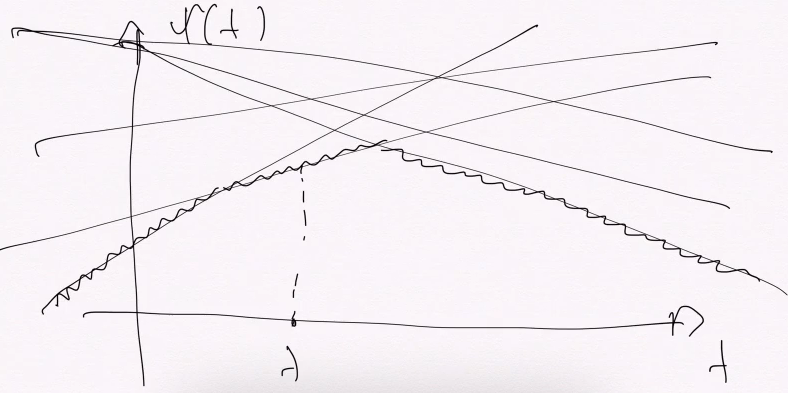
\includegraphics[scale=0.4]{figures/3/chapter3-lagrangian_lines.png}
    \caption{Caption}
    \label{fig:chapter3-lagrangian_lines}
\end{figure}
\par But now bad things: it may happen that the value is $-\infty$ and usually it is not differential, even if all the other stuff is differentiable. But most of all, each time we want to compute the value of the Lagrangian dual, we need to solve a minimisation problem inside. For each $\lambda$ and $\mu$ I clearly have to minimise the Lagrangian relaxed problem.
\par The property $\psi(\lambda,\mu) \leq f(x)$ is called \textbf{weak duality}. We are interested in those cases where we have the equality, i.e. $\psi(\lambda,\mu) = f(x)$, which is called \textbf{strong duality}. Is it always the case that we have the strong duality? Unfortunately no. A counter-example may be:
\begin{align}
    &\min\{-x^2 : 0 \leq x \leq 1\}\\
    &L(x,\lambda,\mu) = -x^2 + \lambda_1 (x-1) + \lambda_2 x\\
    &\psi(\lambda,\mu) = \min \{L(x,\lambda,\mu\} = -\infty, \forall \lambda \in \mathbb{R}^2\\
    &\psi(\lambda,\mu) = -\infty \leq f(x^*) = -1
\end{align}
This is due to the fact that you are minimising a concave function, or maximising a convex function. But under convexity (minimisation) and constraint qualifications, the things work:
\begin{theorem}
    If the problem $P$ is convex, $x^*$ is local optimum and $T_X(x^*) = D_X(x^*)$ (constraint qualifications or regularity), then there exist optimal $\lambda^*, \mu^*$ for the dual problem such that $\psi(\lambda^*, \mu^*) = v(P)$.
\end{theorem}
\begin{proof}
    Since there are optimal $\lambda^*$ and $\mu^*$ for some optimal solution for the problem $P$, $x^*$, we know that the gradient of the Lagrangian function is 0, that is:
    \[
        \nabla_X L(x^*,\lambda^*,\mu^*) = 0
    \]
    It is a saddle point. But since our function is convex, we know that:
    \[
        v(D) \geq \psi(\lambda^*,\mu^*) = \min_{x \in \mathbb{R}^n}\{L(x,\lambda^*,\mu^*)\} = L(x^*,\lambda^*,\mu^*) = f(x^*) = v(P)
    \]
    The first and the second passages are due to the definition. Since we have assumed that the optimal solution is in $x^*$ we get the third passage. Now the forth passage is slightly more involved. Since everything is optimal, KKT conditions are satisfied. So the two large sums in the Lagrangian function become 0 (complementary slackness).
    \par But we also know that the dual optimal value is a lower bound of the optimal value of the primal:
    \[
        v(P) \geq v(D)
    \]
    So it must be the case that the two values are the same:
    \[
        v(P) = v(D)
    \]
\end{proof}
%
\subsection{Specialised duals}
\subsubsection{Linear programs}
\par Dealing with duals and Lagrangian relaxation is not easy. It is a powerful tool, but we need to solve a $\max \min$ problem.
\par There are cases where we can simplify the things a little bit. One of those cases are Linear programs.
\begin{equation}
    \min\{cx : Ax \geq b\}
\end{equation}
Let us compute the Lagrangian function of this problem:
\begin{equation}
    L(x,\lambda) = cx + \lambda(b-Ax) = cx + \lambda b - \lambda Ax = \lambda b + x(c - \lambda A)
\end{equation}
We have obtained a linear function in $x$. The linear function cannot be minimised, it is always $-\infty$. Except one case. The case when the slope of the linear function is 0. That is when we have a constant function. So we get the following:
\begin{equation}
    \psi(\lambda) = \min_{x \in \mathbb{R}^n} L(x,\lambda) =
    \begin{cases}
        -\infty & \mbox{ if } c - \lambda A \neq 0\\
        \lambda b & \mbox{ if } c - \lambda A = 0
    \end{cases}
\end{equation}
So our dual problem becomes:
\begin{equation}
    (D) \max \{\psi(\lambda) : \lambda \geq 0\} \equiv \max \{\lambda b : \lambda A = c, \lambda \geq 0\}
\end{equation}
This is the famous dual of the linear program from operational research.
%
\subsubsection{Quadratic programs}
\par Another interesting special case is the quadratic program. Let us first start with the following one:
\begin{equation}
    \min\{\frac{1}{2}\Vert x \Vert^2 : Ax = b\}
\end{equation}
The Lagrangian relaxation becomes:
\begin{equation}
    L(x,\mu) = \frac{1}{2}\Vert x \Vert^2 + \mu (Ax - b)
\end{equation}
The gradient of the Lagrangian function is then:
\begin{equation}
    \nabla L(x,\mu) = x + \mu A
\end{equation}
Since the gradient of the Lagrangian function must be 0 in the optimum solution, we have that:
\begin{equation}
    \nabla L(x,\mu) = x + \mu A = 0 \rightarrow x = -\mu A
\end{equation}
The dual problem them becomes:
\begin{align}
    \begin{split}\psi(\mu) &= \min_{x \in \mathbb{R}^n} L(x,\mu) = L(-\mu A, \mu) = \frac{1}{2} \Vert -\mu A \Vert^2 + \mu (A(-\mu A) - b) =\\ &=\frac{1}{2} \mu^T AA^T \mu - \mu^T AA^T \mu - b\mu = -\frac{1}{2}\mu^T AA^T \mu - b\mu\end{split}\\
    &\max_{\mu \in \mathbb{R}^n}\Big\{-\frac{1}{2}\mu^T AA^T \mu - b\mu\Big\}
\end{align}
This is a real unconstrained problem.
\par Actually, more generally we could have:
\begin{equation}
    \min \{\frac{1}{2}x^T Q x : Ax \geq b\}
\end{equation}
Under the condition that $A$ is not singular, and thus invertible, we have the following dual problem:
\begin{equation}
    \max\{\lambda b - \frac{1}{2} v^T Q^{-1} v : \lambda A - v = q, \lambda \geq 0\}
\end{equation}
\par All of this is very nice. Imagine that you have a lot of variables, say ten thousands, and very few constraints, say less than 10. Dealing with the dual problem means dealing with a much smaller amount of variables :).
%
\subsubsection{Conic programs}
TODO
%
%
%
\section{Algorithms}
\par We are now going to study some algorithms for solving constrained optimisation programs. In particular we will see three algorithms for solving linearly constrained quadratic programs and two for linearly constrained non linear programs.
\par Thus we will deal with only linear constraints and the difficult part will eventually be the objective function. This is because it is much easier and because this is what we typically do in the machine learning. Sometimes when possible we will do some references to the more general non linear but convex constraints $G(x) \leq 0$. We will exclude non linear and non convex cases. Mainly because of the time limit, but also because they are not that useful in the machine learning world. Typically if you have something that is not linear what you usually do is to approximate the non linear function with something quadratic, e.g. you use Newton. So quadratic programs are quite central.
\par We will not take into account equality constraints because we can always convert them into inequality constraints. Moreover, the problems with only equality constraints we know how to deal with them, since it is almost unconstrained optimisation.
%
\subsection{Equality constraints for quadratic programs}
\par Let us start small. We have already seen quadratic programs with equality constraints. Let us look at it again, this time from the constraint optimisation point of view.
\par Our problem is of the following form:
\begin{equation}
    \min\Big\{\frac{1}{2} x^T Q x + qx : Ax = b\Big\}
\end{equation}
where $A \in \mathbb{R}^{m \times n}$ with $\mbox{rank}(A) = m < n$ and rows of $A$ linearly independent. Note that $Q \succeq 0$ otherwise $v(P) = -\infty$ almost always.
\par Note that since we have just equality constraints, there are no $\lambda$s and thus no complementary slackness condition. The KKT system then becomes:
\begin{align}
    &Ax = b\\
    &\nabla f(x) + \mu \nabla H = Qx + q + \mu A = 0
\end{align}
Which becomes:
\begin{align}
    &Ax = b\\
    &Qx + \mu A = -q
\end{align}
Which can be also written as:
\begin{equation}
    \begin{bmatrix}
    Q & A^T \\
    A & 0
    \end{bmatrix}
    \begin{bmatrix}
    x\\
    \mu
    \end{bmatrix}
    =
    \begin{bmatrix}
    -q\\
    b
    \end{bmatrix}
\end{equation}
This system is symmetric but indefinite. A lot of eigenvalues are 0. This is where Bolzano guy from Pisa comes into play.
\par We could solve this system directly, plain linear algebra. But we can also exploit the particularity of this system in order to craft some efficient methods to solve it. We need to be very efficient since this problem frequently appears as subprogram of a much larger program.
\par One of the possibility is to go by Reduced KKT. If we know that the $Q \succ 0$ then it means that our objective function is strictly convex. We can then do the following. Let us multiply both sides of the main KKT condition by $AQ^{-1}$:
\begin{align}
    &AQ^{-1}Qx + AQ^{-1}A^T\mu = - AQ^{-1}q\\
    &Ax + AQ^{-1}A^T\mu = - AQ^{-1}q\\
    &b + AQ^{-1}A^T\mu = - AQ^{-1}q\\
    &AQ^{-1}A^T\mu = -b - AQ^{-1}q
\end{align}
Let us call $M$ the matrix $AQ^{-1}A^T$. We get the following linear system:
\begin{equation}
    M \mu = - (b + AQ^{-1}q)
\end{equation}
The solution of this system ($\mu$) can be then used to find $x$:
\begin{align}
    &Qx + \mu A^T = -q\\
    &x = Q^{-1}(-A^T \mu - q)
\end{align}
The matrix $M$ is positive semi definite and it is a square matrix ($M \in \mathbb{R}^{m \times m} \wedge M \succeq 0$). This is particularly useful when we have very few constraints ($m$).
\par Another way to solve this problem is the one that we have already examined, Null Space Method. Let us divide $A$ in $[A_B,A_N]$ and $x$ in $[x_B,x_N]$ in a way that $\text{det}(A_B) \neq 0$. In this way $A_B$ is non singular and so we can invert it:
\begin{equation}
    x_B = A_B^{-1}(b - A_N x_N) = A_B^{-1}b - A_B^{-1} A_N x_N
\end{equation}
Let us now call $D = - A_B^{-1} A_N$ and $d = A_B^{-1}b$. We get then:
\begin{equation}
    x_B = D x_N + d
\end{equation}
where:
\begin{equation}
    d = \begin{bmatrix}
    b \\
    0
    \end{bmatrix}
    D = \begin{bmatrix}
    - A_B^{-1} A_N \\
    I
    \end{bmatrix} \in \mathbb{R}^{m \times n - m}
\end{equation}
The matrix $D$ is called the basis of null space of $A$ since we have that:
\begin{equation}
    A D = \begin{bmatrix}
    A_B & A_N \\
    \end{bmatrix} \begin{bmatrix}
    - A_B^{-1} A_N \\
    I
    \end{bmatrix} = - A_B A_B^{-1} A_N + A_N I = - A_N + A_N = 0
\end{equation}
Let us no multiply the KKT main condition by $D^T$:
\begin{equation}
    D^T Q x + D^T A^T \mu = -D^T q
\end{equation}
But since $x = D x_N + d$, the above equality becomes:
\begin{equation}
    D^T Q (D x_N + d) = -D^T q \Rightarrow = (D^T Q D) x_N = -D^T(Q q + d)
\end{equation}
We call $H = D^T Q D \in \mathbb{R}^{n-m \times n-m}$ reduced Hessian and it is positive semi definite.
\par So which method is the best? It depends. Look at the matrices dimensions. If the number of constraints is almost the same as the number of variables then the second one is probably the right choice. If the two numbers are quite different and the number of overall constraints is small, then probably the first one is the one to go.
%
%
%
\section{Projected gradient method}
\par Since the first algorithm that we study for unconstrained optimisation, we will also do the same for the constrained case.
\par This is a method that can be applied to the general non linear objective function with linear constraints:
\begin{equation}
    \min_{x \in \mathbb{R}^n}\{f(x) : Ax \leq b\}
\end{equation}
What we typically do is the line search. So suppose we are in a feasible solution $x$. We want to move in a direction that is feasible. Since everything is linear here (in the sense of the constraints) all the three cones that we have studied are the same. So we need to pick a direction in the first order feasible direction cone $D_X(x)$ restricted to the active constraints:
\begin{equation}
    D_X(x) = \{d \in \mathbb{R}^n : A_{\mathcal{A}(x)}d \leq 0\}    
\end{equation}
We know that the best direction to take is the one of the opposite of the gradient in $x$. So if $\nabla f(x) \in D_X(x)$ then we can just line search on the direction $d = - \nabla f(x)$. Note that if $x$ is in the interior, i.e. $\mathcal{A}_X = \emptyset$ then $D_X(x) = \mathbb{R}^n$, in other words I can go wherever I want.
\par If the gradient does not belong to the set of first order feasible direction cone, then let us find the direction that is as close as possible to the one of the opposite of the gradient. If you think a little bit, the closest direction to $-\nabla f(x)$, which is located outside of the cone, is the direction $d$ that goes along the boundary of the cone on the side of $-\nabla f(x)$.
\par Let us do now some math. We want to project the gradient $\nabla f(x)$ onto $\partial D_X(x)$. Let us describe mathematically the frontier:
\begin{equation}
    \partial D_X(x) = \{d \in \mathbb{R}^n : A_{\mathcal{A}(x)} d = 0\}
\end{equation}
Projection means that we want to minimise the following problem (the closest point, the norm, man):
\begin{equation}
    \min \Big\{\frac{1}{2}\Vert \nabla f(x) - d \Vert^2 = \frac{1}{2} d^T I d - d^T \nabla f(x) : A_{\mathcal{A}(x)}d = 0\Big\}
\end{equation}
This is a linearly constrained quadratic problem with a very special $Q$, that is identity matrix. Note that the identity matrix is strictly positive, that is it is positive definite. So we can use Reduced KKT to solve it in the following manner. First we get $\mu$ by solving this system:
\begin{equation}
    [A_{\mathcal{A}(x)}A_{\mathcal{A}(x)}^T]\mu = A_{\mathcal{A}(x)}\nabla f(x)
\end{equation}
Then we use $\mu$ to find the projected direction:
\begin{equation}
    d = -(A_{\mathcal{A}(x)}^T\mu - \nabla f(x))
\end{equation}
\par Actually, if the matrix of the active constraints in $x$, $A_{\mathcal{A}(x)}$, is non singular, we can also directly get $d$ by doing the following computation:
\begin{equation}
    d = (I - A_{\mathcal{A}(x)}^T(A_{\mathcal{A}(x)}A_{\mathcal{A}(x)}^T)^{-1}A_{\mathcal{A}(x)})\nabla f(x)
\end{equation}
$I - A_{\mathcal{A}(x)}^T(A_{\mathcal{A}(x)}A_{\mathcal{A}(x)}^T)^{-1}A_{\mathcal{A}(x)}$ is called \textbf{projection operator}. This operator projects our nice gradient on the boundary of the feasible region. Remember good old Poloni: householder reflection stuff.
\par So once we have the direction we can do the line search. Almost. $d$ can be also 0. If this is the case, and $\mu \geq 0$ this means that we have found the optimum. Why? Well, look at the original problem. We had $A d \leq 0$. But since our $-\nabla f(x)$ is not a feasible direction, we had to project it by forcing the inequality constraint into the equality constraint. So if there are no $\mu_i$ negative, it means that all the equalities are satisfied. So we are in the optimum. But if $\mu$ is not all positive, then it means that there is a constraint that should not be in the active set $\mathcal{A}_(x)$. We will talk in a minute about that.
\begin{figure}
    \centering
    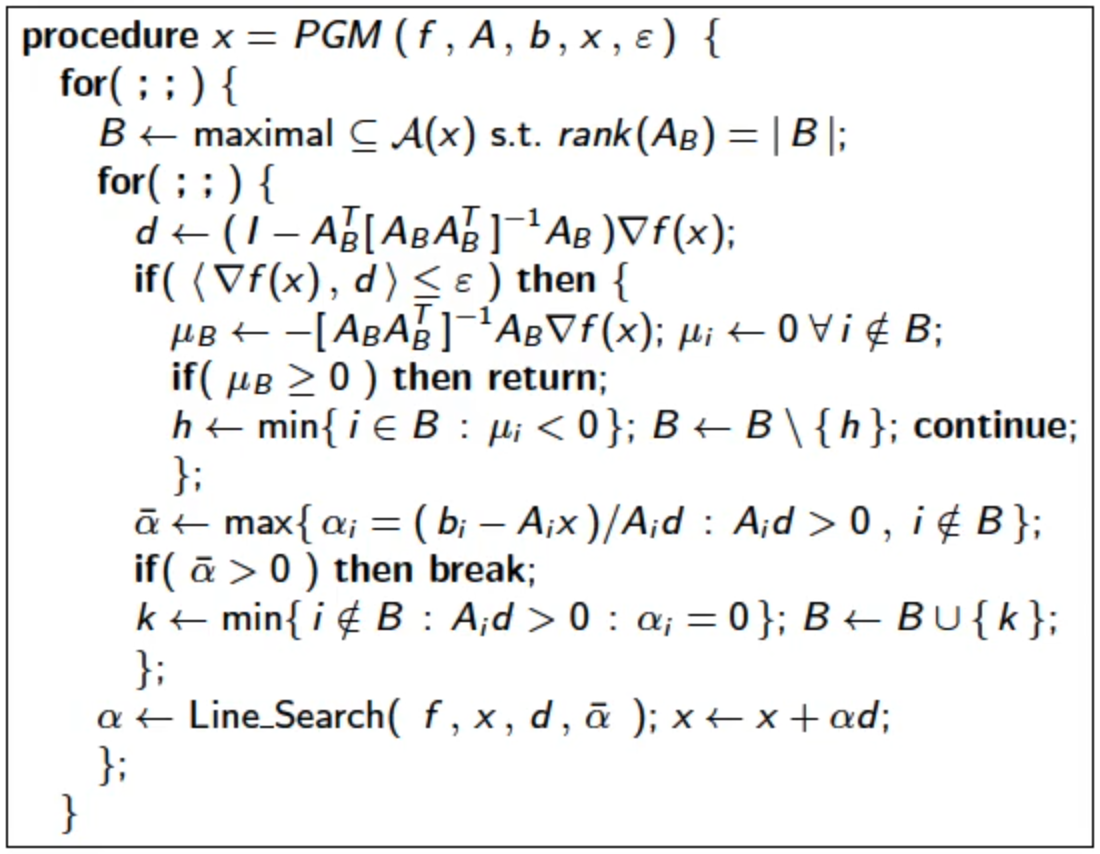
\includegraphics[scale=0.5]{figures/3/chapter3-pgm.png}
    \caption{Projected Gradient Method.}
    \label{fig:chapter3-pgm}
\end{figure}
\par The algorithm is shown in figure \ref{fig:chapter3-pgm}. Let us now go through the algorithm. You start at a point $x$. The first thing that you do is to construct the set of the active constraints in $x$. We take the maximal set of active constraints such that the rank of that set is full rank. We must do this because it is the only way to force non singularity of the matrix $A_B A_B^T$. We annotate that maximal subset of $\mathcal{A}(x)$ with $B$ in the algorithm. Note that we may clearly leave apart some of the active constraints in $x$, and we will have to deal with that. So now we compute the direction $d$. Such direction can either be 0 or not. So if it is 0, then we check if $\mu \geq 0$. We set to 0 all the entries of $\mu$ whose corresponding active constraint has not been included in $B$ previously. In case $\mu \geq 0$, we are done. Otherwise we find the entry with negative value in $\mu$ that has the lowest index and we throw from $B$ the corresponding constraint. Yes. We just ignore it. And we repeat. Two cases eventually happen. Either we end up again with $d = 0$ and the whole process repeats until we get out from the whole procedure because we hit $\mu \geq 0$ or we find a $d \neq 0$. In this last case we proceed in the algorithm. Since we left some of the constraints out of the set $B$ we now must verify that the direction that we found does not violate some of the constraints out of $B$. We take the step size along each such constraint and then we take the minimum of those values. If the minimum is greater than 0, it means we can proceed along $d$. If $d \leq 0$ it means that some of the constraints is active but not in $B$. So we include that constraint and we repeat.
\par Let us now state without proving some of the properties about PGM. First of all, the addition of the constraints in $B$ preserve the linear independence. That is we do not risk to make $B$ singular. It is also not possible to have the add/remove process cyclical. That is the process of addition and removal of constraints eventually terminates. This is called \textbf{Bland's anti-cycle rule}. Maximal $B$ is easy to get, just do the greedy algorithm. Each constraint either we put it or not in $B$ depending on whether it is linearly independent from all the constraints already belonging to $B$. How? For each matrix that you form with a new vector, check that the determinant of that matrix is not 0.
\par Note that if $f$ is a simple linear function, then PGM is just the \textbf{Primal Simplex Method}.
\par Sometimes in ML the constraints are much easier than the general constraints. One of the easiest types of constraints is called \textbf{box constraints}. Each variable belongs to an interval of values, $l \leq x \leq u$. If we have a non linear program with box constraints, the algorithm becomes much more simpler (see figure \ref{fig:chapter3-pgm_box}).
\begin{figure}
    \centering
    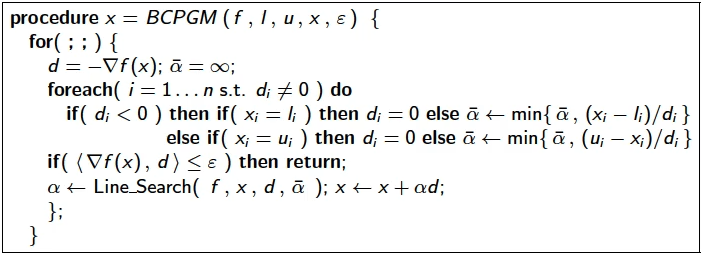
\includegraphics[scale=0.4]{figures/3/chapter3-pgm_box.png}
    \caption{Projected Gradient Method with Box Constraints.}
    \label{fig:chapter3-pgm_box}
\end{figure}
\par For each box constraint, if it is active then $x$ is either $l$ or $u$. So the set of active constraints is always linearly independent. How this algorithm works? We start with the direction opposite of the gradient. For each entry $i$ of the direction vector $d$ that is $\neq 0$ (remember, we want $d$ to be 0 in order to terminate), we do the following: if $d_i < 0$ we need to lower a bit $x_i$. But if $x_i = l_i$ we just set it to 0 since we cannot go anymore down. Otherwise we calculate the minimum step size for the new direction by taking the minimum between the previous minimum step sizes and the current one. The same process applies for $d_i > 0$.
%
%
%
\section{Active-set method for Quadratic Programming with linear inequalities}
\par Suppose now we have a quadratic program with linear inequalities. If we knew which were the active constraints in the optimal solution $x^*$ we would just apply linear algebra and the world would be a better place. But unfortunately we don't know that. We like, especially in ML, to guess when we don't know exactly the things. We need also to be prepared to also revise our estimates.
\par The algorithm is shown in figure \ref{fig:chapter3-asmqp}. Let us go through it. The first thing that we note is that we do not require that the matrix $B$ contains just linearly independent set of active constraints. Note that this set can also be empty, i.e. $B = \emptyset$. What we do then is to solve the linear equality constrained quadratic program. Note that we are hiding the concept of $B$ being full rank inside that subroutine. The rest is quite straightforward. If $\bar{x}$ is a feasible solution, then we have found the optimum if $\mu_B \geq 0$. Note that we know that it is optimal on $A_B$, so we need to check only the constraints not in $B$. If this is not the case we proceed as in the case of the projected gradient method. The only thing to say here is that as you can see we do not need to do any line search. This is because we are in the case of the quadratic program. We can just take the maximum step size in the descent direction.
\begin{figure}
    \centering
    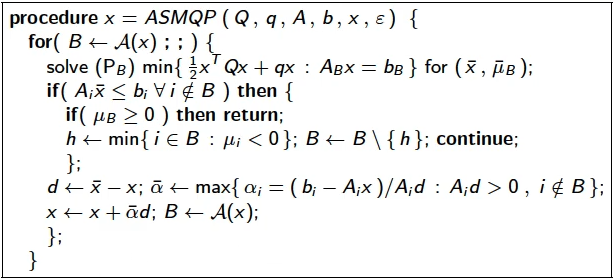
\includegraphics[scale=0.4]{figures/3/chapter3-asmqp.png}
    \caption{Active set method for quadratic programming}
    \label{fig:chapter3-asmqp}
\end{figure}
\par This method can be also extended to $f$ general, that is not necessarily quadratic. What changes is how we solve the subproblem. We could use for instance quasi-Newton.
TODO box contraints
%
%
%
\section{Frank Wolfe method, aka Conditional Gradient}
\par The main difficulty with projected gradient method and active set method is the active set. Frank Wolfe tries to do without it at all. We will deal here with non linear programs with linear constraints. 
\begin{figure}
    \centering
    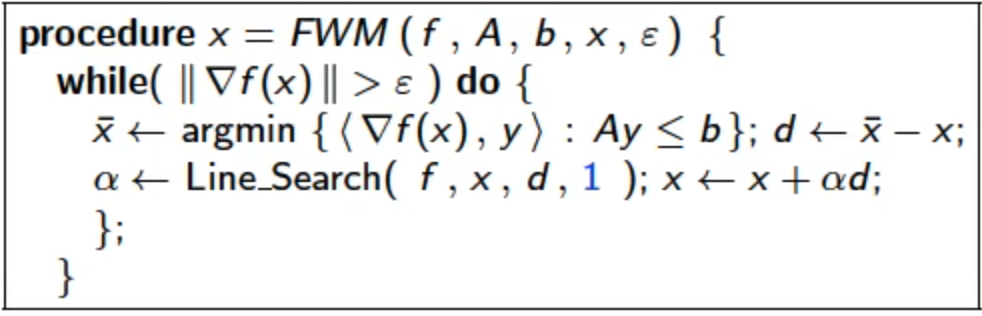
\includegraphics[scale=0.5]{figures/3/chapter3-fwm.png}
    \caption{Frank Wolfe Method, also called Conditional Gradient Method.}
    \label{fig:chapter3-fwm}
\end{figure}
\par The idea of Frank Wolfe is quite simple (figure \ref{fig:chapter3-fwm}. It assumes there is someone else that can deal with the linear problem and let us concentrate only on the non linear part of the problem which is in the objective function. It iteratively approximate the our nasty function with the first order linear model, minimise this program in the admissible region and take that direction as the direction of descent.
\par Another thing worth mentioning is that we do not need to compute the maximum step size. We just set it to 1.
\par This algorithm is particularly easy to implement but unfortunately it is not that good when it comes to the convergence. This is because we trust the linear model on the whole admissible region. It is accurate locally to $x$ but probably this is not the case when we look at the whole admissible region. What we can do to improve the convergence is the stabilisation.
TODO
%
%
%
\section{Dual Methods}
\par Frank Wolfe completely hides Lagrangian multipliers. Suppose again we have a quadratic program with linear constraints.